\documentclass[8pt]{beamer}
% \usepackage[utf8]{inputenc} is no longer required (since 2018)

%Set the font (output) encoding
%--------------------------------------
\usepackage[T1]{fontenc} %Not needed by LuaLaTeX or XeLaTeX

%French-specific commands
%--------------------------------------
\usepackage[french]{babel}
\usepackage[autolanguage]{numprint} % for the \nombre command

%Hyphenation rules
%--------------------------------------
\usepackage{hyphenat}
\hyphenation{mate-mática recu-perar}
%--------------------------------------
\usepackage{amsmath}
\usepackage{bm}
\usepackage{subcaption}
\usepackage{tikz}

% Theme choice
\usetheme[block=fill, sectionpage=none, progressbar=frametitle,
    numbering=none]{metropolis}

\usecolortheme{orchid}

% Title, author, and date information
\title{Gestion de la Mémoire dans les Systèmes Informatiques}
\subtitle{Hiérarchie Mémoire et Pagination}
\author{Yohan Chatelain}
\institute{Polytechnique Montr\'eal}
\date{1 Juin 2024}

\begin{document}

% Title slide
\begin{frame}
    \titlepage
\end{frame}

\begin{frame}{Plan du cours}
    \begin{block}{Objectifs : }

        \begin{itemize}
            \item Les différents types de mémoires
            \item La hiérarchie mémoire (Pourquoi et Comment ?)
            \item Principe de localité (temporelle et spatiale)
            \item La gestion de la mémoire (virtuelle et physique)
            \item La pagination
        \end{itemize}
    \end{block}
\end{frame}

\addtocounter{framenumber}{-2}
\setbeamertemplate{frame numbering}[fraction]

\section*{Introduction}
\begin{frame}
    \frametitle{Introduction}
    \begin{itemize}
        \item La mémoire est le deuxième composant majeur de tout ordinateur
    \end{itemize}
    \begin{figure}
        \centering

        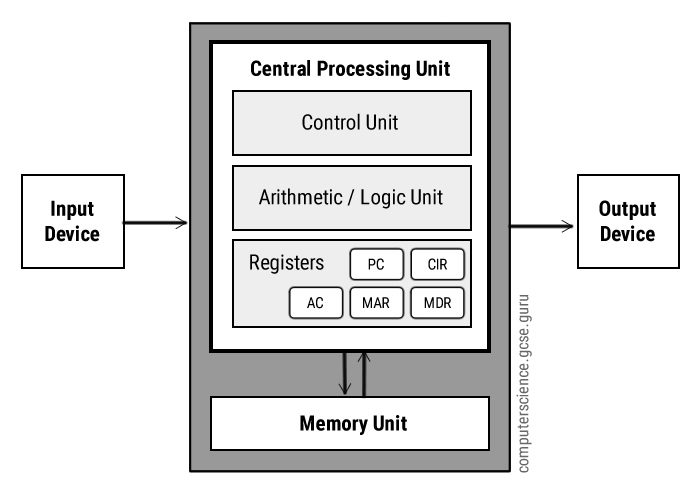
\includegraphics[width=.45\textwidth]{figures/Von-Neumann-Architecture-Diagram.jpg}
        \subcaption{Architecture de Von Neumann~\cite{tanenbaum2009modern}}
        \label{fig:sub1}
    \end{figure}
    \begin{block}{La mémoire idéale devrait être :}
        \begin{itemize}
            \item Extrêmement rapide
            \item Très grande capacité
            \item Peu coûteuse
        \end{itemize}
    \end{block}

\end{frame}

\begin{frame}{Spoiler alert!}
    \begin{figure}
        \centering
        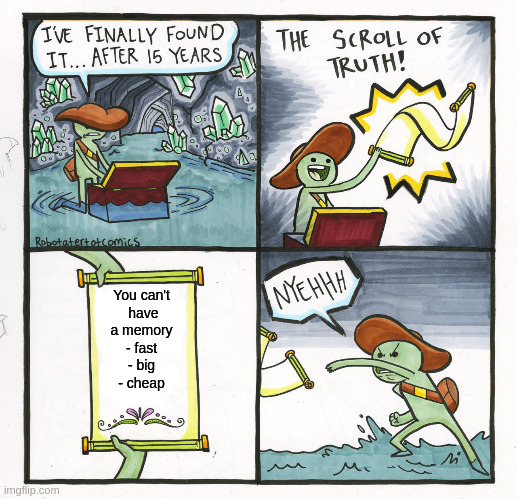
\includegraphics[width=0.5\textwidth]{figures/meme.jpg}
        \label{fig:memory_speed}
    \end{figure}

    \begin{alertblock}{Problème}
        \begin{itemize}
            \item La technologie actuelle ne satisfait pas tous ces objectifs
        \end{itemize}
    \end{alertblock}
\end{frame}

\begin{frame}{Cons\'equences}
    \begin{figure}[ht]
        \centering
        \centering
        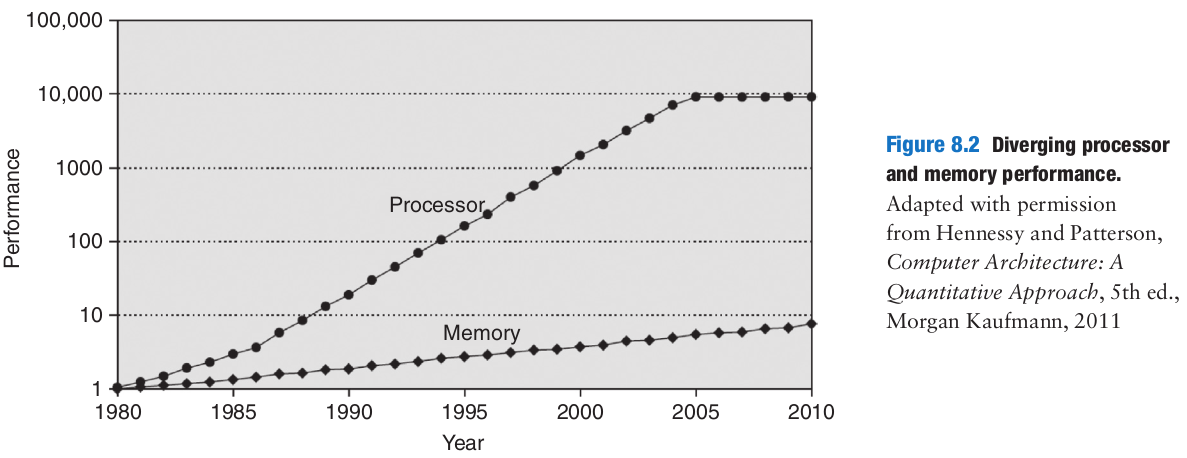
\includegraphics[width=.75\linewidth]{figures/gap_cpu_ram_H.png}
        \subcaption{\'Ecart de performance entre CPU et
            RAMS~\cite{harris2021digital}}
        \label{fig:sub2}
    \end{figure}
    \begin{itemize}
        \item La performance des CPUs double tous les $1,5$ ans (loi de Moore),
              \\ celles des mémoires tous les $\simeq5$ ans
        \item Les \'echanges de données entre la mémoire et le CPU sont
              lents.
              \begin{itemize}
                  \item Ordre de grandeur : $\boldsymbol{\times}\textbf{100}$
                        \textbf{plus
                            lent}
                        pour
                        accéder
                        à la RAM qu'aux registres
              \end{itemize}
        \item Les acc\`es mémoire sont nombreux et fréquents dans les
              programmes
        \item Ils representent le \textbf{principale goulet d'\'etranglement}
    \end{itemize}
\end{frame}

\begin{frame}
    \frametitle{Hiérarchie Mémoire}

    \begin{alertblock}{Questions :}
        \begin{itemize}
            \item Quelles types de memoires connaissez-vous ?
            \item Quelle est le r\^ole de chacune de ces m\'emoires ?
        \end{itemize}
    \end{alertblock}
\end{frame}

\begin{frame}
    \frametitle{Les différent types de mémoires}
    \begin{block}{Principe général}

        Plus une m\'emoire est rapide, plus elle est ch\`ere \`a
        fabriquer, plus sa taille est limit\'ee
    \end{block}
    \begin{enumerate}
        \item \textbf{Registre} : Mémoire très rapide, très coûteuse et
              volatile. \\
              Contient les données de travail des unités de calculs.
        \item \textbf{Cache} : Mémoire rapide, coûteuse et volatile. \\
              Contient les données et instructions les plus utilisées par les
              unités de calculs.
              %   ($ \simeq 1-100 \$ / MB$)
        \item \textbf{Centrale} : Mémoire de vitesse moyenne, coût moyen et
              volatile. \\
              Contient les données et instructions des programmes en cours
              %   ($ \simeq 2-20 \$ / GB$)
        \item \textbf{Stockage} : Mémoire lente, peu coûteuse et non volatile
              . \\
              Contient les données et instructions des programmes non utilisés
              \\
              (disques magnétiques/SSD)
              %   ($ \simeq 0.05-2 \$ / GB$)
    \end{enumerate}

\end{frame}

\begin{frame}{Hiérarchie mémoire}
    \begin{block}{Principe de localité}
        Les programmes ont tendance à accéder aux \textbf{données} et
        \textbf{instructions} :
        \begin{enumerate}
            \item plusieurs fois \`a la suite (\textbf{localité temporelle})
            \item proches les unes des autres (\textbf{localité spatiale})
        \end{enumerate}
        Il convient donc de garder les données fréquemment utilisées rapidement
        accessible pour le CPU
    \end{block}
    \begin{itemize}
        \item Le système de mémoire est construit comme une hiérarchie
              de
              couches
        \item Chaque type de m\'emoire r\'epond \`a un objectif en
              terme de
              rapidit\'e/taille/co\^ut
    \end{itemize}

    \begin{figure}
        \centering
        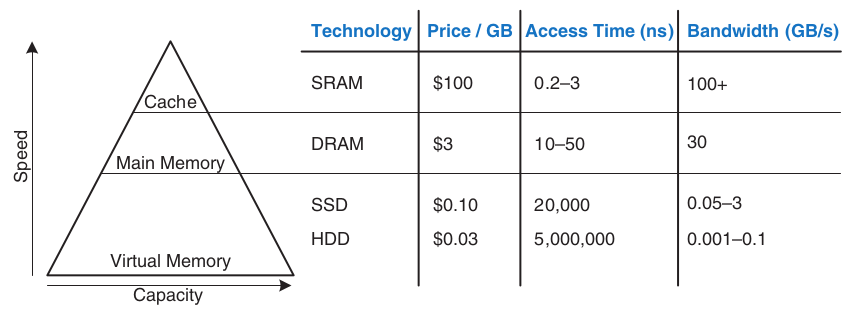
\includegraphics[width=.75\textwidth]{figures/memory_speed_HH.png}
        \caption{Hiérarchie de la mémoire \cite{harris2021digital}}
    \end{figure}

\end{frame}

\begin{frame}<presentation:0>[noframenumbering]
    \frametitle{Registres}
    \begin{itemize}
        \item Premiere couche de la hiérarchie mémoire, integr\'es au CPU.
        \item Extrêmement rapides sans délai d'accès.
        \item Très faible capacité (moins de 4 Ko).
        \item Deux types de registres : instructions et données.
        \item Utilisés pour stocker les données de travail des unites de
              calculs.
    \end{itemize}
    \begin{figure}
        \centering

        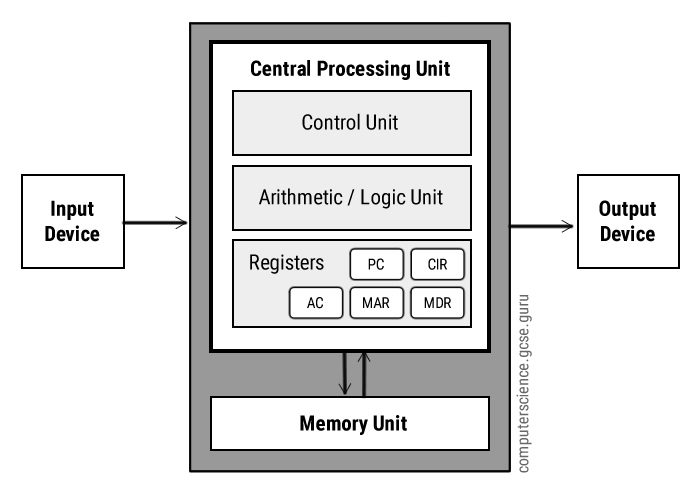
\includegraphics[width=.45\textwidth]{figures/Von-Neumann-Architecture-Diagram.jpg}
        \subcaption{Architecture de Von Neumann~\cite{tanenbaum2009modern}}
        \label{fig:sub1}
    \end{figure}

\end{frame}
\begin{frame}<presentation:0>[noframenumbering]
    \frametitle{Mémoire Cache}
    \begin{itemize}
        \item Taille limitée en raison de son coût élevé (SRAM \$\$\$)
        \item Divisée en lignes de cache correspondant \`a la m\'emoire
              principale
        \item Hiérarchique, avec plusieurs niveaux de cache
        \item Principalement contrôlée par le matériel ($\to$ Le\c{c}on X sur
              les caches)
    \end{itemize}
\end{frame}
\begin{frame}
    \frametitle{Mémoire Cache}
    \begin{block}{Principes}
        \begin{itemize}
            \item \textbf{Hiérarchie} : Les niveaux de cache sont organisés en
                  hiérarchie, du plus rapide et plus petit au plus lent et plus
                  grand
            \item \textbf{Redondance} : Les données stockées dans un niveau de
                  cache
                  sont également stockées dans les niveaux de cache supérieurs
            \item \textbf{Localité} : Les données stockées dans un niveau de
                  cache
                  inferieur sont celles qui sont les plus susceptibles d'être
                  utilisées par le CPU
        \end{itemize}
    \end{block}
    \begin{figure}
        \centering
        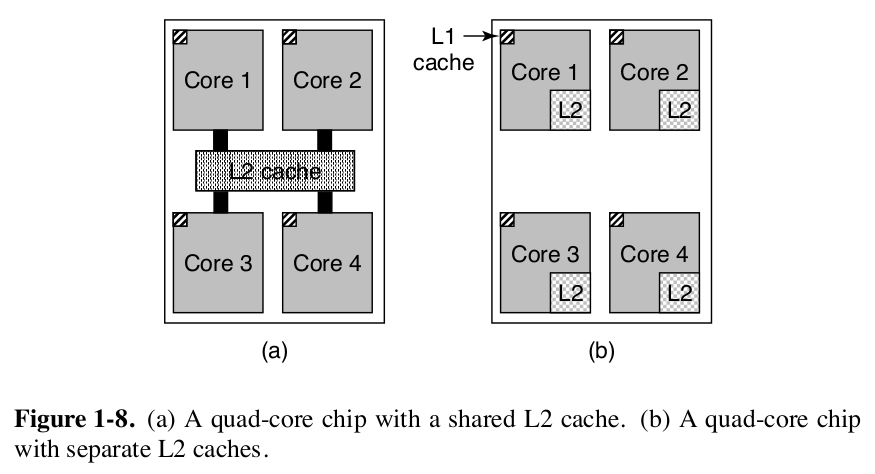
\includegraphics[width=.6\textwidth]{figures/ProcCoresCache_T.png}
        \subcaption{Mémoire cache~\cite{tanenbaum2009modern}}
    \end{figure}
    \begin{tikzpicture}[remember picture, overlay]
        \node[anchor=south west, inner sep=0pt] at
        ([shift={(0.1cm,0.1cm)}]current page.south west)
        {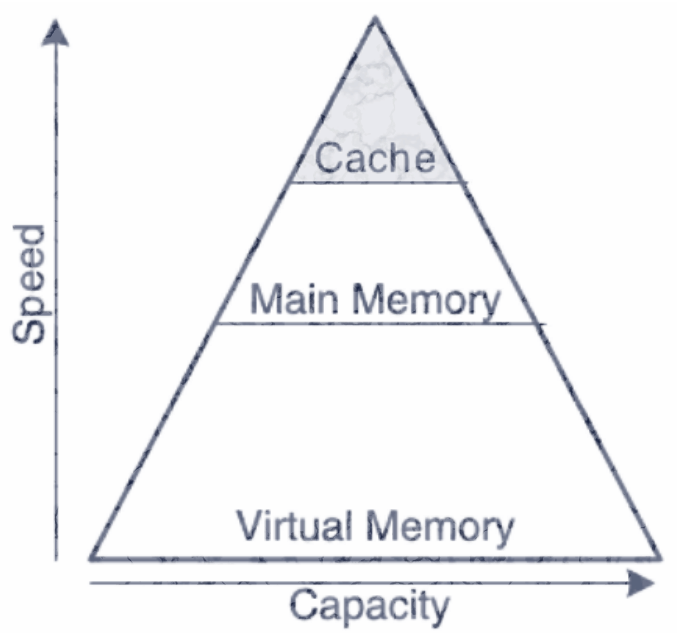
\includegraphics[alt={text},
                width=0.15\textwidth]{figures/pyramid_layout_cache.png}};
    \end{tikzpicture}

\end{frame}

\begin{frame}{title}
\end{frame}

\begin{frame}<presentation:0>[noframenumbering]
    \frametitle{Composition d'une Mémoire Cache}
    \begin{block}{Composition d'une ligne de cache}
        \begin{itemize}
            \item \textbf{Données} : Contenu de la mémoire principale
            \item \textbf{Étiquette} : Adresse de la mémoire principale
            \item \textbf{Bits de contrôle} : Informations de contrôle
                  (Explain)
        \end{itemize}
    \end{block}
    \begin{figure}
        \centering
        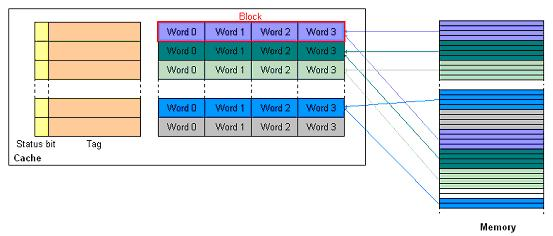
\includegraphics[width=.5\textwidth]{figures/Direct_mapped_cache.JPG}
        \subcaption{Mémoire cache à correspondance préétablie (direct-mapped
            cache) [Wikipedia]}
    \end{figure}
    \vspace*{-.5cm}
    \begin{block}{Principe de fonctionnement}
        \begin{itemize}
            \item \textbf{Vérification} : Toutes les opérations mémoires
                  passent d'abord par la mémoire cache.
            \item \textbf{Succès (Hit)} : Si donnée présente, transmise
                  au processeur.
            \item \textbf{Défaut (Miss)} : Si donnée absente, transférée
                  de la mémoire principale à la mémoire cache.
        \end{itemize}
    \end{block}
\end{frame}

\begin{frame}
    \frametitle{Mémoire Principale}
    \begin{block}{Mémoire Physique (RAM)}
        \begin{itemize}
            \item Contient les \textbf{données} et \textbf{instructions} des
                  programmes en cours d'exécution
            \item Peut contenir des dizaines de Go dans les
                  systèmes modernes
            \item \textbf{Mémoire volatile} : les données sont perdues lorsque
                  l'alimentation est coupée
            \item \textbf{Accès lent} par rapport à la mémoire cache
        \end{itemize}
    \end{block}
    \begin{figure}
        \centering
        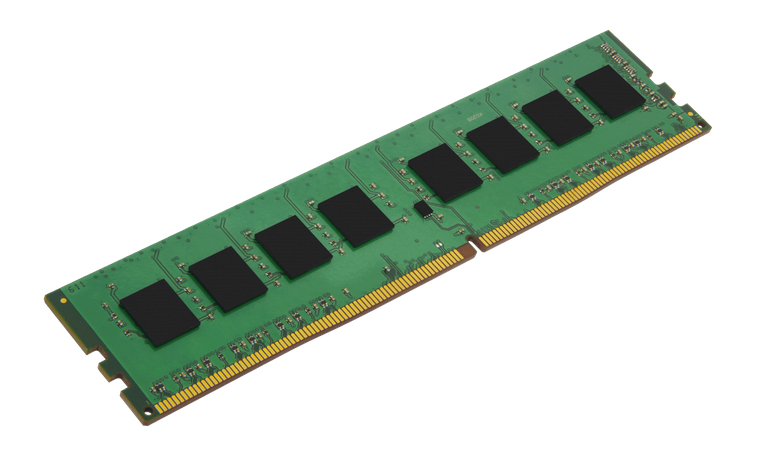
\includegraphics[width=.5\textwidth]{figures/DRAM.png}
        \subcaption{DRAM [TechTerms]}
    \end{figure}
    \begin{tikzpicture}[remember picture, overlay]
        \node[anchor=south west, inner sep=0pt] at
        ([shift={(0.1cm,0.1cm)}]current page.south west)
        {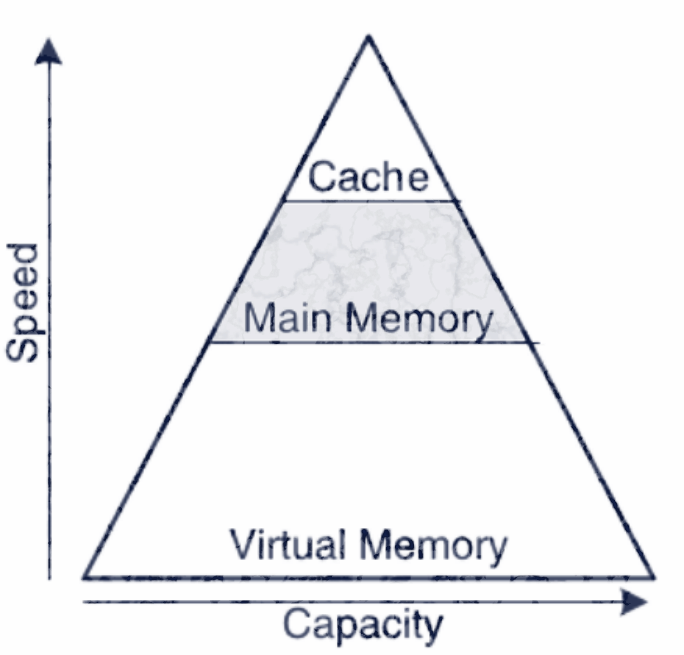
\includegraphics[alt={text},
                width=0.15\textwidth]{figures/pyramid_layout_main.png}};
    \end{tikzpicture}
\end{frame}

\begin{frame}{Est-ce suffisant ?}
    \begin{figure}
        \centering
        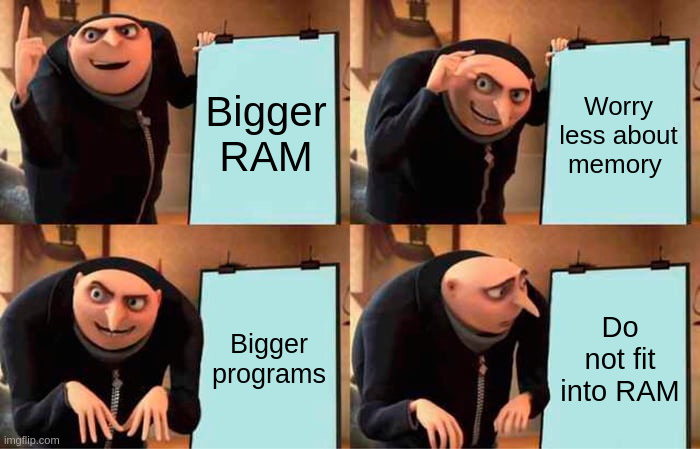
\includegraphics[width=.75\textwidth]{figures/RAM_meme.jpg}
    \end{figure}
\end{frame}

\begin{frame}
    \frametitle{Mémoire Virtuelle}
    \begin{block}{Principe}
        \begin{itemize}
            \item Permet de "virtuellement" d'allouée plus de mémoire que la
                  capacité mémoire physique
            \item Fournie l’illusion d’un \textbf{espace mémoire
                      contigu} de
                  grande
                  taille au programmeur.
            \item Chaque processus \`a son \textbf{propre espace
                      d'adresses}
            \item \textbf{Abstraction} decoup\'ee en blocs de taille
                  fixe appel\'es \textbf{pages}
            \item Gérée par l'Unité de Gestion de Mémoire
                  (\emph{\textbf{M}emory
                      \textbf{M}anagement \textbf{U}nit})

        \end{itemize}
    \end{block}
    \begin{example}
        \begin{itemize}
            \item Architecture 16bits : $2^{16}$ adresses possibles, soit 64Ko
                  (1Ko=$2^{10}$o) addressable virtuellement
            \item Une configuration de 32Ko de RAM + 64Ko de disque
            \item Memoire physique : 32Ko RAM, Memoire virtuelle : 64Ko
            \item Espace d'adressage 32Ko = $32 \times 2^{10} = 2^5
                      \times2^{10} = 2^{15}$o $\to$ 15 bits n\'ecessaires
        \end{itemize}
    \end{example}
    \begin{tikzpicture}[remember picture, overlay]
        \node[anchor=south west, inner sep=0pt] at
        ([shift={(0.1cm,0.1cm)}]current page.south west)
        {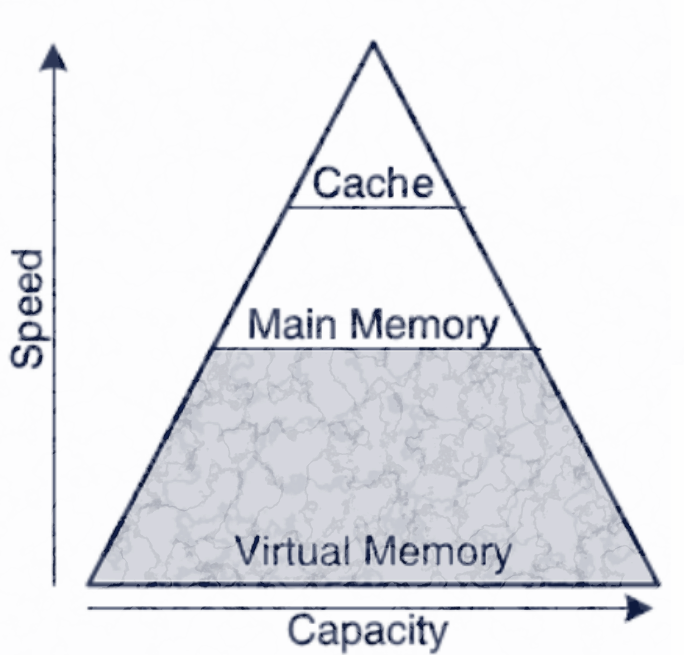
\includegraphics[alt={text},
                width=0.15\textwidth]{figures/pyramid_layout_virtual.png}};
    \end{tikzpicture}
\end{frame}

\begin{frame}[c]
    \frametitle{Mémoire Virtuelle - Illustration}
    \begin{onlyenv}<1>
        \vspace*{1.25cm}
        \begin{figure}
            \centering
            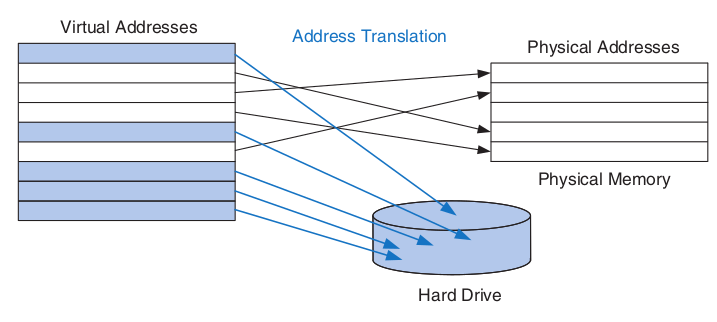
\includegraphics[width=.9\textwidth]{figures/vir.png}
            \subcaption{Diagramme de la mémoire
                virtuelle et la mémoire physique~\cite{harris2021digital}}
        \end{figure}
    \end{onlyenv}
    \begin{onlyenv}<2->
        \begin{figure}
            \centering
            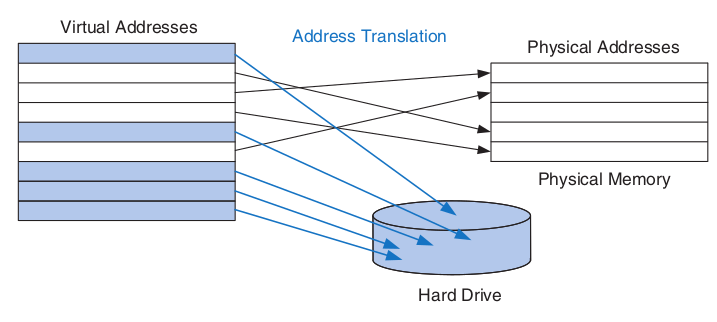
\includegraphics[width=.5\textwidth]{figures/vir.png}
            \subcaption{Diagramme de la mémoire
                virtuelle et la mémoire physique~\cite{harris2021digital}}
        \end{figure}
    \end{onlyenv}
    \pause
    \begin{alertblock}{Question : }
        \begin{itemize}
            \item
                  Quelle est l'avantage du d\'ecoupage en page ?
        \end{itemize}
    \end{alertblock}
    \pause
    \begin{exampleblock}{Solution : La pagination}
        \begin{itemize}
            \item Une application \textbf{n'utilise pas toute la mémoire} qui
                  lui est
                  allouée en même
                  temps
            \item Charger en mémoire \textbf{uniquement les pages nécessaires}
                  à
                  l'exécution
            \item Principe de \textbf{localité} similaire \`a la m\'emoire
                  cache
        \end{itemize}
    \end{exampleblock}

\end{frame}

\begin{frame}<presentation:0>[noframenumbering]
    \frametitle{Mémoire de Masse}
    \begin{block}{Principes}
        \begin{itemize}
            \item \textbf{Stockage non-volative} : les données sont conservées
                  même lorsque l'alimentation est coupée
            \item \textbf{Accès lent} aux données par rapport à la mémoire
                  principale
            \item \textbf{Assurer la fiabilité} et la durabilité des données
                  stockées.
            \item \textbf{Stockage de grandes quantités de données} (plusieurs
                  To)

        \end{itemize}
    \end{block}
    \begin{exampleblock}{Types de mémoire de masse}
        \begin{itemize}
            \item Disques durs (Hard Disk Drive)
            \item Disques à état solide (Solid State Drive)
            \item Disques optiques (CD-ROM)
            \item Bandes magnétiques (Grande capacité de plusieurs Po, faible
                  coût)
        \end{itemize}
    \end{exampleblock}
    \begin{figure}
        \centering
        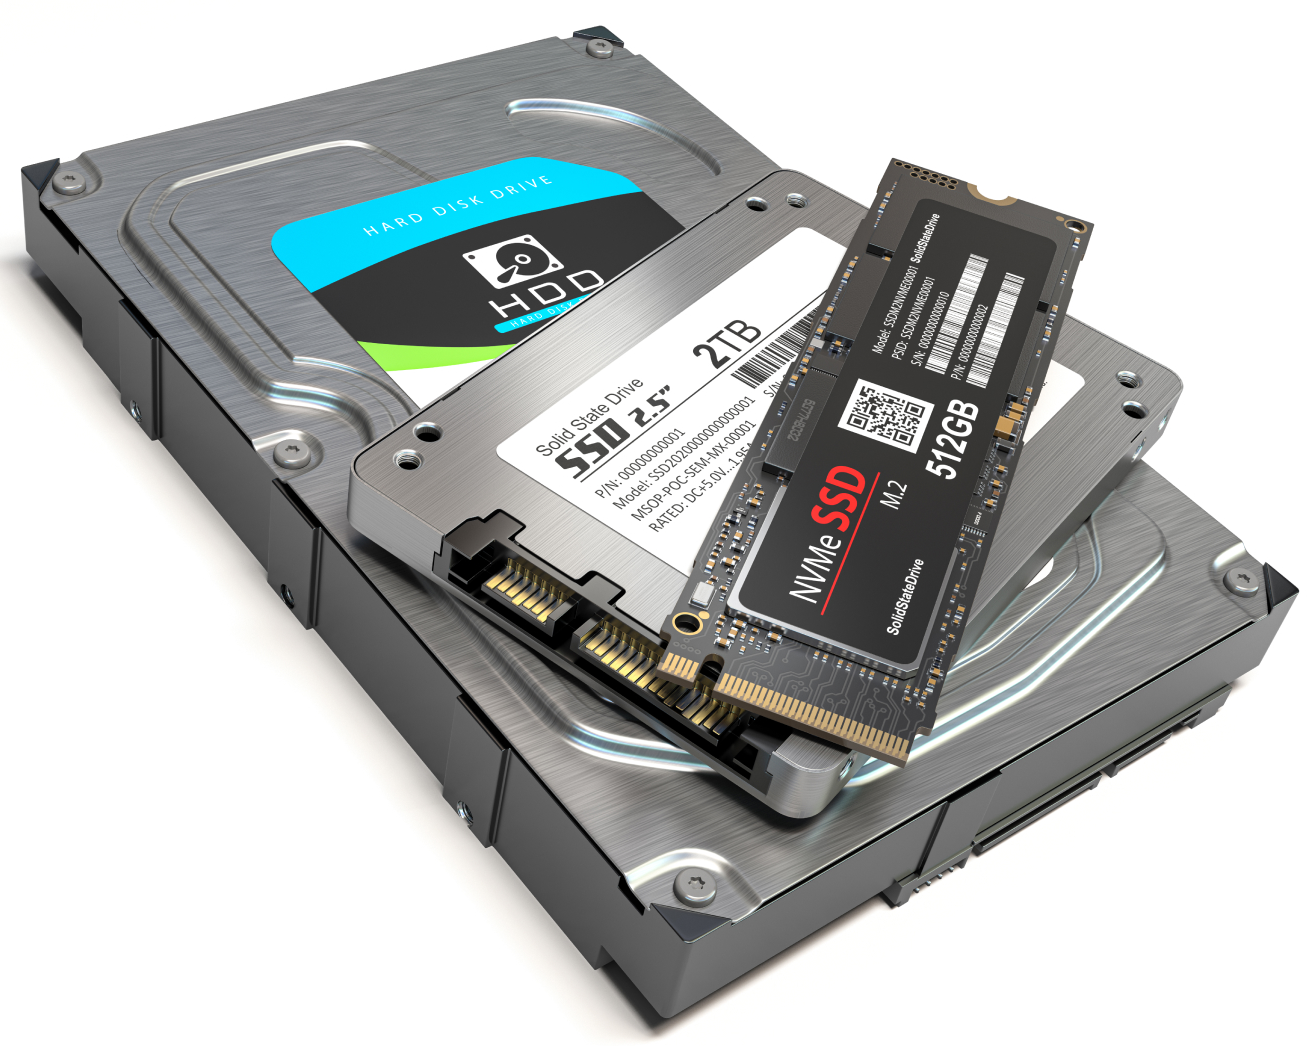
\includegraphics[width=.25\textwidth]{figures/HDD+SSD.png}
        \subcaption{HDD, SSD et NVMe-SSD [NZXT]}
    \end{figure}
\end{frame}

\begin{frame}{Pagination}
    \begin{block}{Principe}
        \begin{itemize}
            \item Un processus \textbf{n'utilise pas toute la mémoire} qui
                  lui est
                  allouée en même
                  temps
            \item Charger en mémoire \textbf{uniquement les pages nécessaires}
                  à
                  l'exécution
            \item Principe de \textbf{localité} similaire \`a la m\'emoire
                  cache
        \end{itemize}
    \end{block}
    \begin{block}{D\'efinition}
        \begin{itemize}
            \item \textbf{Pagination} : Division de la mémoire virtuelle en
                  blocs de taille fixe appelés \textbf{pages}
            \item \textbf{Page} : Bloc de mémoire virtuelle de taille fixe
                  (4-64 Ko)
                  \textbf{pages}
            \item \textbf{Tables de Pages} : Associe les pages
                  virtuelles aux pages physiques
            \item \textbf{MMU} : Traduction des adresses virtuelles en
                  adresses physiques
            \item \textbf{TLB} : Cache pour accélérer la
                  traduction (\emph{\textbf{T}ranslation \textbf{L}ookaside
                      \textbf{B}uffer})
        \end{itemize}
    \end{block}
\end{frame}

\begin{frame}
    \frametitle{Table des pages et Traduction}
    \begin{figure}
        \begin{minipage}[b]{0.45\linewidth}
            \centering
            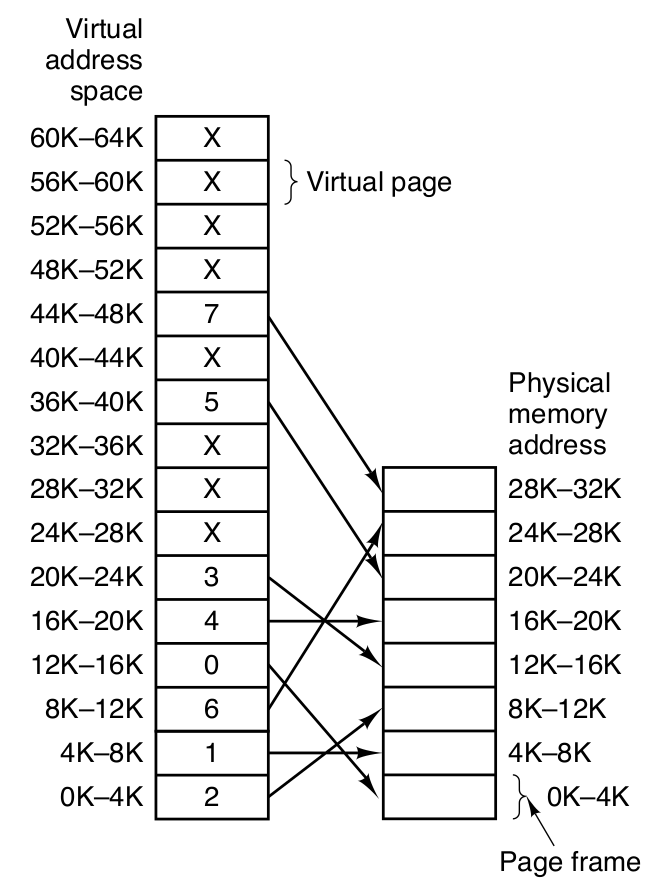
\includegraphics[width=.75\linewidth]{figures/page_table_wo.png}
            \subcaption{}
            \label{fig:page_table}
        \end{minipage}
        \begin{minipage}[b]{0.5\linewidth}
            \centering
            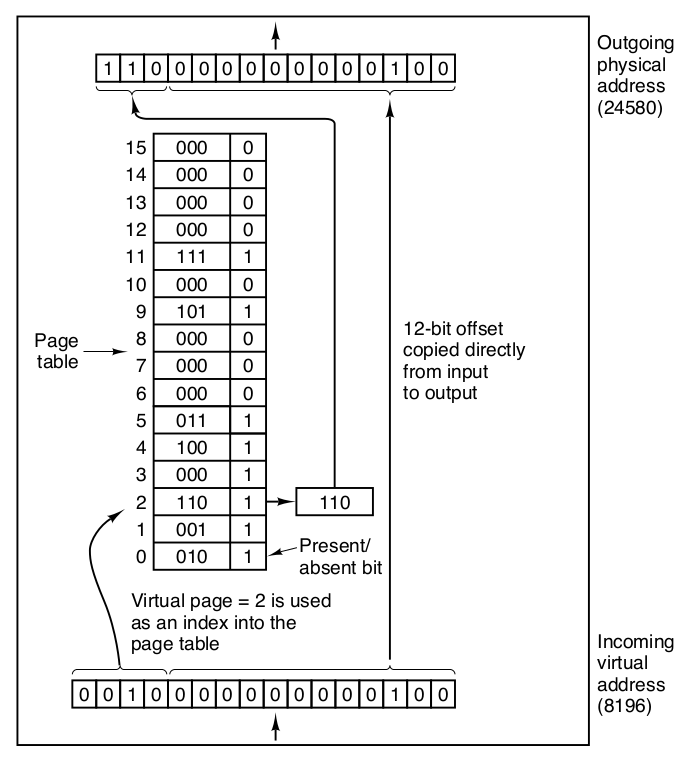
\includegraphics[width=.75\linewidth]{figures/page_mapping.png}
            \subcaption{}
            \label{fig:page_mapping}
        \end{minipage}
        \caption{Table des pages simplifiée pour une architecture 16 bits avec
            un bit de
            pr\'esence. \\ (a) Table des pages et (b) Traduction mémoire
            virtuelle vers
            physique (MMU)~\cite{tanenbaum2009modern}. \\
            Architecture 16 bits,
            Mémoire Virtuelle : 64Ko, Mémoire Physique : 32Ko,
            Taille de page : 4Ko. \\
        }
    \end{figure}
    $\to$ Le\c{c}on X pour des tables des pages plus complexe.

    % \includegraphics[width=\linewidth]{memory_mapping_example}
\end{frame}

\begin{frame}
    \frametitle{Translation Lookaside Buffer (TLB)}

    \begin{alertblock}{Problème de performance}
        \begin{itemize}
            \item La traduction doit \^etre rapide pour \'eviter
                  l'attente du
                  CPU.
            \item Ce qui r\'eduit la taille de la table des pages
            \item \textbf{Localité} : le même petit nombre de pages est souvent
                  utilisées par un processus.
        \end{itemize}
    \end{alertblock}
    \begin{exampleblock}{Solution}
        \begin{itemize}
            \item \textbf{TLB} : Cache de traduction d'adresses
            \item Stocke les traductions récentes, taille de quelques 10 à 1000
                  entrées
            \item Vérifie d'abord le TLB avant de chercher dans la table des
                  pages
        \end{itemize}
    \end{exampleblock}
    \begin{figure}
        \centering
        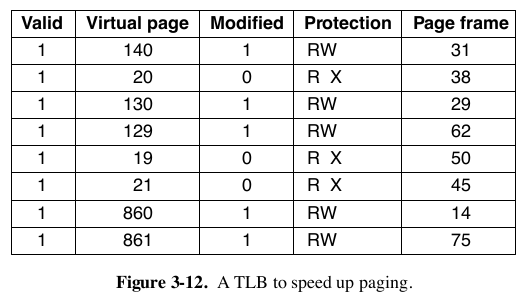
\includegraphics[width=.35\textwidth]{figures/TLB.png}
        \subcaption{Translation Lookaside Buffer~\cite{tanenbaum2009modern}}
    \end{figure}
    % \includegraphics[width=\linewidth]{memory_management_diagram}
\end{frame}

\begin{frame}{Conclusion}
    \begin{block}{Mémoire dans les systèmes informatiques}
        \begin{itemize}
            \item La hiérarchie mémoire est une solution aux
                  contraintes de \\\textbf{rapidité}, \textbf{capacité} et
                  \textbf{coût}
            \item La \textbf{localité} est un principe fondamental pour la
                  gestion
                  de la
                  mémoire
            \item \textbf{Mémoire virtuelle} : Vision unifiée de la
                  mémoire pour les programmes
            \item \textbf{Pagination} : Division de la mémoire en
                  pages pour gérer la
                  localité
            \item La \textbf{table des pages} (MMU) traduit les adresses
                  virtuelles en adresses physiques
            \item Les \textbf{caches} et les \textbf{TLB} sont des éléments
                  clés pour accélérer
                  l'accès à la mémoire
        \end{itemize}
    \end{block}
    \begin{exampleblock}{Prochaines leçons}
        \begin{itemize}
            \item Politiques de placement dans les caches
            \item Politiques de remplacement et d'\'ecriture dans les caches
            \item Tables de pages avancées (multi-niveaux, inversion de pages)
            \item Algorithmes de remplacement de pages
        \end{itemize}
    \end{exampleblock}
\end{frame}

\bibliographystyle{apalike}
\begin{frame}{Bibliographie}
    \nocite{*}
    \bibliography{main}
\end{frame}
\addtocounter{framenumber}{-1}

\end{document}
